\documentclass[economies,article,submit]{Definitions/mdpi}

\usepackage{amsmath}
\usepackage{amssymb}
\usepackage{booktabs}
\usepackage{threeparttable}
\usepackage{longtable}
\usepackage{array}
\usepackage{graphicx}
\usepackage{float}
\usepackage{ragged2e}

\graphicspath{{figures/}}
\renewcommand{\arraystretch}{0.95}
\setlength{\tabcolsep}{4pt}

\firstpage{1}
\makeatletter
\setcounter{page}{\@firstpage}
\makeatother
\pubvolume{1}
\issuenum{1}
\articlenumber{0}
\pubyear{2026}
\copyrightyear{2026}
\externaleditor{Firstname Lastname}
\datereceived{}
\daterevised{}
\dateaccepted{}
\datepublished{}

\Title{Nonlinear Effects of Digital Factor Allocation on Regional Coordinated Development: Evidence from a Provincial Panel Threshold Model in China}

\newcommand{\orcidauthorA}{0009-0004-5051-4277}
\newcommand{\orcidauthorB}{0009-0005-2206-6857}
\newcommand{\orcidauthorC}{0009-0008-3195-5631}
\Author{Junfeng Wang \orcidA{}, Jiayi Wang \orcidB{} and Yile Wang *\orcidC{}}
\AuthorNames{Junfeng Wang, Jiayi Wang and Yile Wang}
\address[1]{School of Marxism, Beijing Technology and Business University, Beijing 100048, China; eventhat@btbu.edu.cn (J.W.)\\
Digital College, Beijing Technology and Business University, Beijing 100048, China; 2401050126@st.btbu.edu.cn (J.W.)\\
School of Economics, Beijing Technology and Business University, Beijing 100048, China; 2401050128@st.btbu.edu.cn (Y.W.)\
Correspondence: 2401050128@st.btbu.edu.cn}
\corres{\hangafter=1 \hangindent=1.05em \hspace{-0.82em}Correspondence: 2401050128@st.btbu.edu.cn}

\abstract{China's digital economy has grown rapidly, but whether digital factor allocation promotes regional coordinated development remains an open question. This study constructs a digital factor allocation (DFA) index covering digital infrastructure, digital industry, digital finance, and digital human capital, and a regional coordinated development (RCD) index covering economic, social, and urban-rural coordination for 30 Chinese provinces from 2013 to 2021. Using the entropy weight method and a Hansen panel threshold model, this study examines the nonlinear relationship between DFA and RCD. The results show that DFA is positively associated with RCD: the baseline two-way fixed-effects estimate is 0.241 (p < 0.05). The association is nonlinear. When per capita GDP exceeds the estimated threshold of 10.589 (about CNY 39,700), the marginal association rises from 0.506 to 0.677. A financial development threshold indicates that the marginal association declines at very high levels of financial depth, consistent with diminishing returns to digital finance. The association is strongest in western provinces, and channel analysis suggests that industrial upgrading, financial deepening, and technological investment are plausible mechanisms. These findings imply that digital factor policies should be sequenced with economic development, tailored to regional absorptive capacity, and accompanied by complementary reforms in advanced regions.}

\keyword{digital factor allocation; regional coordinated development; threshold effect; absorptive capacity; digital finance; China}

\begin{document}

\section{Introduction}\label{sec:intro}

Over the past decade, China has built one of the world's largest digital economies. Broadband networks, mobile payments, e-commerce platforms, and cloud-based public services have expanded from leading coastal cities into inland and rural areas. This expansion has changed how firms organize production, how households access finance and markets, and how governments deliver public services \citep{goldfarb2019}. Yet the gains have not been evenly distributed. Per capita income, public-service capacity, and digital infrastructure remain uneven across provinces, and the gap between leading and lagging regions is a central concern of China's regional policy \citep{zhangky2019,worldbank2009}.

Digital factor allocation (DFA)---the combined availability and application of digital infrastructure, digital industry, digital finance, and digital human capital across regions---is a potential lever for regional coordinated development (RCD). Digital infrastructure lowers the cost of market access and information diffusion; digital finance extends payment, credit, and insurance services to households and small firms that were previously excluded; digital industry creates new employment and productivity opportunities; and digital human capital determines whether these opportunities are absorbed locally \citep{czernich2011,hjort2019,jack2014,zhang2019}. In this sense, DFA can support economic coordination, social coordination, and urban-rural coordination, the three core dimensions of RCD.

The same forces can also widen regional gaps. Digital investment tends to cluster where complementary skills, finance, and infrastructure are already available \citep{forman2012,akerman2015}. Platform markets reward scale and concentration, and automation can displace routine labor in regions that are least able to adjust \citep{acemoglu2020,autor2018}. Rural and lagging regions may gain access to digital services but lack the capability to convert access into productivity and income gains \citep{vandijk2005,norris2001,warschauer2003}. Whether DFA promotes or undermines RCD is therefore an empirical question, and the answer may depend on the stage of economic development and the local absorptive capacity.

Existing research on digitalization and regional development can be grouped into three strands. The first strand focuses on measurement. Studies construct digital economy indices from internet penetration, related employment, digital output, mobile internet, and digital financial inclusion \citep{zhao2020,guo2020}. These indices are useful for ranking regions, but they often aggregate heterogeneous digital factors into a single score and do not distinguish infrastructure, industry, finance, and human capital. The second strand examines the effects of digitalization on growth, productivity, employment, and inclusion \citep{czernich2011,hjort2019,huang2019,zhang2019}. The evidence is broadly positive, but the estimated effects vary across settings and are often sensitive to the level of development. The third strand introduces nonlinearity. Threshold models show that digitalization can have stage-dependent effects, with the marginal effect changing once a critical level of digital development, market efficiency, or technological progress is reached \citep{qi2025}. These studies suggest that linear estimates may mask important heterogeneity.

Three gaps remain. First, most studies use a composite digital economy index and do not examine whether the effect of DFA depends on complementary economic conditions. A composite index can be dominated by leading provinces and can obscure the separate roles of infrastructure, industry, finance, and human capital. Second, RCD is often measured by a single indicator, such as GDP growth or the urban-rural income ratio, rather than by a multidimensional index that reflects economic, social, and urban-rural coordination. Third, the threshold evidence for China is still limited, and the mechanisms through which DFA affects RCD are not well identified.

To fill these gaps, this study constructs a multidimensional DFA index and a multidimensional RCD index for 30 Chinese provinces from 2013 to 2021. The DFA index covers digital infrastructure, digital industry, digital finance, and digital human capital. The RCD index covers economic coordination, social coordination, and urban-rural coordination. Both indices are constructed with the entropy weight method, which avoids subjective weighting and preserves the information content of the underlying indicators. The study then applies a Hansen panel threshold model to examine whether the effect of DFA on RCD changes once economic development or financial development crosses a critical level. The analysis also examines regional heterogeneity and three plausible channels: industrial upgrading, financial deepening, and technological investment.

The contributions of this study are fourfold. (1) \textbf{Measurement}: It develops a transparent DFA index that distinguishes four digital factor categories and an RCD index that covers three coordination dimensions, allowing the analysis to move beyond a single composite score. (2) \textbf{Nonlinear identification}: It uses a panel threshold model to test whether the DFA effect depends on economic development and financial development, and it reports bootstrap tests and likelihood-ratio confidence intervals for the threshold estimates. (3) \textbf{Regional and channel evidence}: It shows how the effect varies across regions and identifies industrial upgrading, financial deepening, and technological investment as plausible channels. (4) \textbf{Policy relevance}: It provides a differentiated policy framework that sequences digital factor allocation with economic development and complementary reforms.

The results show that DFA is positively associated with RCD. Under two-way fixed effects, a one-unit increase in the DFA index is associated with an increase of 0.241 points in the RCD index (p < 0.05). The association is nonlinear. When per capita GDP exceeds the estimated threshold of 10.589 (about CNY 39,700), the marginal association rises from 0.506 to 0.677. A financial development threshold indicates that the marginal association declines at very high levels of financial depth, consistent with diminishing returns to digital finance. The association is strongest in western provinces, and the channel analysis suggests that industrial upgrading, financial deepening, and technological investment are plausible mechanisms. These findings are consistent with an absorptive-capacity interpretation: digital factor allocation is most effective when local economic conditions allow digital inputs to be combined with complementary skills, markets, and institutions.

The remainder of this paper is organized as follows. Section~\ref{sec:lit} reviews the literature and develops the hypotheses. Section~\ref{sec:data} describes the data, indices, and empirical strategy. Section~\ref{sec:results} reports the results. Section~\ref{sec:discussion} discusses the findings, policy implications, and limitations. Section~\ref{sec:conclusion} concludes.

\section{Literature Review and Hypotheses}\label{sec:lit}

\subsection{Digital Factor Allocation and Regional Coordinated Development}

Regional coordinated development refers to the joint improvement of economic performance, social welfare, and urban-rural balance across regions, not simply the convergence of GDP per capita. It also requires that public services, income opportunities, and basic infrastructure be accessible in different locations and that the gains from growth be shared between leading and lagging areas \citep{kanbur2005,worldbank2009}. In China, RCD has been pursued through fiscal transfers, infrastructure investment, poverty alleviation, and, more recently, digitalization.

DFA can affect RCD through four channels. Digital infrastructure reduces communication and transaction costs, allowing firms in lagging regions to reach customers and information that were previously available only in core regions \citep{czernich2011,hjort2019}. Digital finance extends payment, savings, credit, and insurance to households and small firms, improving risk sharing and relaxing liquidity constraints \citep{jack2014,beck2007,liu2023}. Digital industry creates new tasks and raises productivity in services that are less dependent on physical distance \citep{goldfarb2019,acemoglu2011}. Digital human capital determines whether local workers can use digital tools productively \citep{akerman2015,vandijk2005}.

This reasoning supports a positive relationship, but the empirical literature also cautions that the benefits are conditional. Forman et al. (2012) show that the internet's wage effects are concentrated in already prosperous areas, and Akerman et al. (2015) find that broadband complements skilled labor. Whether DFA has a uniform effect across Chinese regions is therefore an open question.

\subsection{Absorptive Capacity and Threshold Effects}

The idea that digitalization has stage-dependent effects comes from the absorptive-capacity literature. Digital technologies are general-purpose technologies whose effects depend on how they are combined with organizational change, human capital, and institutional quality \citep{brynjolfsson2014,omahony2005}. In low-income regions with thin markets, digital inputs may be used for consumption rather than productive investment; in higher-income regions the same inputs can be combined with skills, finance, and infrastructure to generate larger coordination gains. This predicts that the marginal effect of DFA increases with economic development.

Hansen (1999) provides a fixed-effects panel threshold estimator that lets the slope of a regressor differ across regimes defined by an observed variable, searching for the threshold that minimizes the residual sum of squares and testing linearity by bootstrap. The approach has been extended to instrumental-variable and dynamic panels \citep{caner2004,seo2016} and is widely used on Chinese regional data. Qi et al. (2025), for example, find threshold effects of digital development, market efficiency, and technological progress on Chinese-style modernization, which suggests that the digital dividend depends on the broader development environment.

The threshold interpretation also connects to the digital divide. Access is only the first level; the second and third levels concern skills and the ability to convert access into material benefits \citep{vandijk2005,norris2001,warschauer2003}. If the second and third divides persist in low-income regions, the effect of DFA on RCD may be weak there and stronger once complementary capabilities are in place.

\subsection{Financial Development and Diminishing Returns}

Digital finance is a core component of DFA, and its effect may depend on the depth of the financial system. Where financial development is limited, digital finance substitutes for missing branches and expands access to basic services. Where the system is already deep, it adds less at the extensive margin, may intensify competition, or may divert resources from productive investment. The relationship between financial depth and inclusion is therefore unlikely to be linear \citep{beck2007}. Digital finance has expanded fastest in leading cities where financial services were already abundant, so its marginal contribution to RCD may be larger where finance is scarce. This motivates a second threshold in financial development.

\subsection{Regional Heterogeneity and Mechanisms}

China's regions differ in initial digital endowments, industrial structure, and institutional capacity. The east has denser digital infrastructure, more high-skilled labor, and deeper financial markets; the centre and west start lower but may have more room for catch-up; the northeast carries a heavy-industry legacy and a slow digital transition. The absorptive-capacity argument predicts a stronger effect in the east, whereas the catch-up argument predicts a stronger effect in the west. The two can be distinguished empirically.

Three mechanisms are relevant. DFA can promote industrial upgrading by reducing information costs, expanding market access, and enabling new service activities \citep{chen2025,rodrik2016}. It can deepen financial development by extending the coverage and use of digital financial services \citep{chen2025,liu2023}. And it can raise technological investment by lowering the cost of innovation-related information and creating demand for digital skills \citep{akerman2015}. The channel analysis in this study is exploratory.

\subsection{Hypotheses}

\textbf{H1.} Digital factor allocation is positively associated with regional coordinated development.

\textbf{H2.} The effect of DFA on RCD is nonlinear; the marginal effect is larger after economic development crosses a threshold, consistent with absorptive capacity.

\textbf{H3.} The effect of DFA varies with financial development and tends to diminish at very high levels of financial depth.

\textbf{H4.} The effect of DFA is regionally heterogeneous, with a stronger average effect in less-developed western provinces.

\textbf{H5.} DFA promotes RCD through industrial upgrading, financial deepening, and technological investment.

\begin{figure}[H]
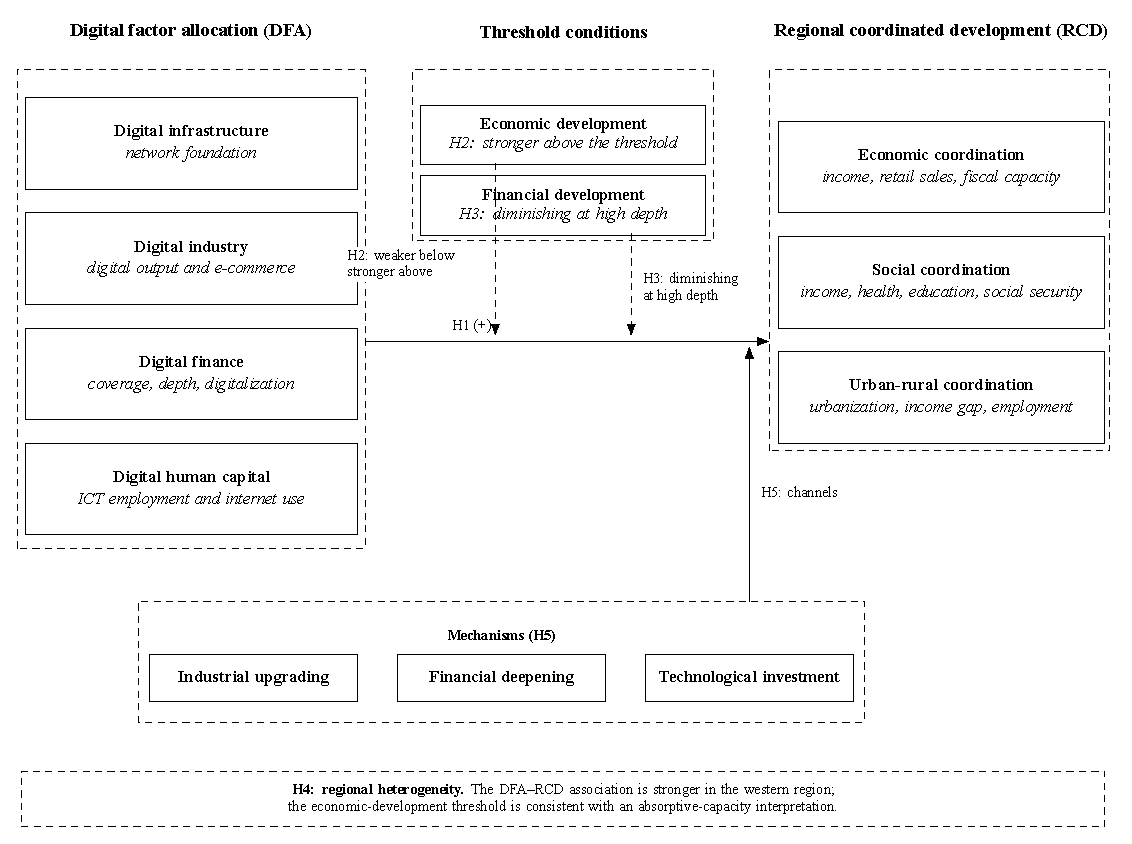
\includegraphics[width=0.95\textwidth]{figures/fig1_framework_tikz.pdf}
\caption{Research framework. DFA is measured across four dimensions and RCD across three dimensions. H1 tests the average association; H2 tests whether the DFA slope differs across economic-development regimes; H3 examines the financial-development threshold; H4 summarizes regional heterogeneity; H5 examines the channels.}\label{fig:framework}
\end{figure}

\section{Data, Variables, and Methods}\label{sec:data}

\subsection{Study Area and Data}

The analysis covers 30 provincial-level units in mainland China from 2013 to 2021. Tibet, Hong Kong, Macao, and Taiwan are excluded because of data availability and comparability. The panel is balanced with 270 observations. The sample starts in 2013 because the National Bureau of Statistics introduced a unified urban-rural household survey that year, which makes the income series comparable over the period.

Provincial economic, social, infrastructure, and environmental indicators are taken from the \emph{China Statistical Yearbook} (2014--2022), the \emph{China City Statistical Yearbook} (2014--2022), the \emph{China Environmental Statistics Yearbook}, and provincial yearbooks \citep{nbs2022,nbscity2022}. Digital financial inclusion sub-indices come from the Peking University Digital Financial Inclusion Index \citep{pku2021}. A small number of missing values were filled by linear interpolation within provinces. For urban and rural incomes, we checked the extracted values against the accounting identity linking total disposable income to urban and rural incomes and the urbanization rate, and corrected cells that violated it.

\subsection{Digital Factor Allocation Index}

DFA is measured with a four-dimension system (Table~\ref{tab:indicators}). Digital infrastructure captures the network foundations that determine whether digital services reach firms and households; digital industry captures the scale and market application of digital production; digital finance captures the coverage, intensity, and digitalization of financial services; and digital human capital captures the supply of workers who can use digital technologies.

The 15 indicators are selected for relevance to the dimension, availability across all provinces and years, and consistency of definitions. To prevent a few large provinces from dominating the index, indicators are expressed as per capita, per GDP, or per area ratios. DFA assigns equal weights to the four dimensions and entropy weights to indicators within each dimension, so each factor category has the same ex ante importance while the data determine the weights inside it.

\subsection{Regional Coordinated Development Index}

RCD is measured with a three-dimension system (Table~\ref{tab:indicators}). Economic coordination uses GDP per capita, retail sales per capita, and fiscal self-sufficiency. Social coordination uses disposable income per capita, hospital beds per 10,000 people, higher-education students per 100,000 people, and the share of social security spending. Urban-rural coordination uses the urbanization rate, the urban-rural income ratio (negative), and the urban registered unemployment rate (negative).

The three dimensions receive equal weights and entropy weights are applied within each dimension. For robustness we also construct a five-dimension index that adds infrastructure and ecological coordination, a coupling coordination degree for the three core dimensions, and a global entropy-weighted index.

\begin{table}[htbp]
\caption{Indicator systems for digital factor allocation (DFA) and regional coordinated development (RCD).}\label{tab:indicators}
\footnotesize
\begin{tabular}{>{\raggedright\arraybackslash}p{3.0cm}>{\raggedright\arraybackslash}p{4.2cm}>{\raggedright\arraybackslash}p{5.0cm}c}
\toprule
Dimension & Indicator & Definition and unit & Sign \\
\midrule
\multicolumn{4}{l}{\textit{Panel A: Digital factor allocation (DFA)}} \\
\midrule
Digital infrastructure & Internet access ports per capita & Internet broadband access ports / year-end population (ports per person) & + \\
 & Optical cable density & Long-distance optical cable length / land area (km/km$^2$) & + \\
 & Mobile phone penetration & Mobile phone subscribers per 100 people & + \\
 & IPv4 addresses per capita & IPv4 addresses / year-end population & + \\
 & Domain names per capita & Registered domain names / year-end population & + \\
Digital industry & Software revenue / GDP & Software business revenue / GDP (\%) & + \\
 & E-commerce sales / GDP & E-commerce transaction value / GDP (\%) & + \\
 & Firms with e-commerce & Share of enterprises with e-commerce transactions (\%) & + \\
 & Websites per 100 firms & Number of websites per 100 enterprises & + \\
 & Information firms per capita & Information enterprises / year-end population & + \\
Digital finance & DFI coverage breadth & Peking University Digital Financial Inclusion Index sub-index & + \\
 & DFI usage depth & Peking University Digital Financial Inclusion Index sub-index & + \\
 & DFI digitization & Peking University Digital Financial Inclusion Index sub-index & + \\
Digital human capital & ICT employment share & Employment in information transmission, computer services, and software / total urban employment (\%) & + \\
 & Internet penetration & Internet users / year-end population (\%) & + \\
\midrule
\multicolumn{4}{l}{\textit{Panel B: Regional coordinated development (RCD)}} \\
\midrule
Economic coordination & GDP per capita & Regional GDP / year-end population (CNY/person) & + \\
 & Retail sales per capita & Retail sales of consumer goods / year-end population (CNY/person) & + \\
 & Fiscal self-sufficiency & Local fiscal revenue / local fiscal expenditure (\%) & + \\
Social coordination & Disposable income per capita & All residents' per capita disposable income (CNY/person) & + \\
 & Hospital beds & Hospital beds per 10,000 people & + \\
 & Higher-education students & Higher-education students per 100,000 people & + \\
 & Social security spending & Social security and employment expenditure / fiscal expenditure (\%) & + \\
Urban-rural coordination & Urbanization rate & Urban resident population / year-end population (\%) & + \\
 & Urban-rural income ratio & Urban disposable income / rural disposable income & $-$ \\
 & Urban unemployment rate & Registered urban unemployment rate (\%) & $-$ \\
\bottomrule
\end{tabular}

\noindent\footnotesize Notes: All indicators are compiled from the \emph{China Statistical Yearbook}, the \emph{China City Statistical Yearbook}, provincial statistical yearbooks, and the Peking University Digital Financial Inclusion Index. DFA assigns equal weights to the four dimensions and entropy weights to indicators within each dimension. RCD assigns equal weights to the three dimensions and entropy weights to indicators within each dimension.
\end{table}

\subsection{Entropy Weight Method}

The entropy method assigns larger weights to indicators with greater dispersion. For indicator $j$ and observation $i$, the raw value $x_{ij}$ is winsorized at the 1st and 99th percentiles and normalized. For positive indicators,
\begin{equation}
z_{ij}=\frac{x_{ij}-\min_i x_{ij}}{\max_i x_{ij}-\min_i x_{ij}},
\end{equation}
and for negative indicators,
\begin{equation}
z_{ij}=\frac{\max_i x_{ij}-x_{ij}}{\max_i x_{ij}-\min_i x_{ij}}.
\end{equation}
A constant ($10^{-4}$) is added to avoid zeros. The normalized values become proportions $p_{ij}=z_{ij}/\sum_i z_{ij}$, and the entropy of indicator $j$ is
\begin{equation}
e_j=-\frac{1}{\ln N}\sum_{i=1}^{N}p_{ij}\ln p_{ij},
\end{equation}
where $N$ is the number of observations. The weight is
\begin{equation}
w_j=\frac{1-e_j}{\sum_{k}(1-e_k)},
\end{equation}
and the composite score is $S_i=\sum_j w_j z_{ij}$. Entropy weights are computed within each dimension and the dimension scores are averaged with equal weights, which prevents a dimension with many indicators from receiving disproportionate weight.

\subsection{Baseline and Threshold Models}

The baseline specification is a two-way fixed-effects model:
\begin{equation}
RCD_{it}=\alpha_0+\alpha_1 DFA_{it}+\gamma'X_{it}+\mu_i+\delta_t+\varepsilon_{it},
\label{eq:baseline}
\end{equation}
where $i$ indexes provinces, $t$ indexes years, $\mu_i$ and $\delta_t$ are province and year fixed effects, $X_{it}$ is a vector of controls, and $\varepsilon_{it}$ is clustered at the province level.

To test H2 and H3 we estimate a Hansen (1999) panel threshold model:
\begin{equation}
RCD_{it}=\beta_0+\beta_1 DFA_{it}\cdot I(q_{it}\leq\gamma)
+\beta_2 DFA_{it}\cdot I(q_{it}>\gamma)
+\gamma'X_{it}+\mu_i+\varepsilon_{it},
\label{eq:threshold}
\end{equation}
where $q_{it}$ is the threshold variable and $I(\cdot)$ is the indicator function. The threshold is estimated by grid search over the inner 80\% of the distribution of $q$. The null of linearity is tested with a cluster wild bootstrap that generates $y^*=\hat{y}+\varepsilon^*$, where $\varepsilon^*$ is the fitted residual multiplied by a province-level Rademacher sign, and re-estimates the threshold and the $F$ statistic in each replication. The $p$-value is the share of bootstrap statistics above the observed one. We also report the likelihood-ratio confidence interval for $\gamma$ using the critical value 7.35 \citep{hansen1999,hansen2000}.

The threshold variable is economic development (log GDP per capita) for H2 and financial development for H3. We also estimate specifications using DFA, technological investment, and private economy vitality as threshold variables to check whether the nonlinearity is specific to economic development.

\subsection{Controls and Descriptive Statistics}

The controls capture local conditions that may affect RCD but are not part of the index. Government intervention is local expenditure over GDP; foreign direct investment is log realized FDI per capita; population density is log year-end population per square kilometer; and private economy vitality is private enterprises per 10,000 people. Together they cover the fiscal, external, spatial, and market dimensions of local conditions.

Table~\ref{tab:descriptives} reports descriptive statistics. DFA has a mean of 0.259 and a standard deviation of 0.179; RCD has a mean of 0.357 and a standard deviation of 0.148. The urban-rural income ratio averages 2.53 and ranges from 1.84 to 3.56.

\begin{table}[htbp]
\caption{Descriptive statistics.}\label{tab:descriptives}
\begin{threeparttable}
\small
\begin{tabular}{lrrrrrr}
\toprule
Variable & N & Mean & SD & Min & Median & Max \\
\midrule
DFA index & 270 & 0.259 & 0.179 & 0.007 & 0.223 & 1.000 \\
RCD index & 270 & 0.357 & 0.148 & 0.083 & 0.333 & 0.846 \\
RCD5 index & 270 & 0.414 & 0.117 & 0.137 & 0.406 & 0.805 \\
RCD coupling coordination & 270 & 0.555 & 0.180 & 0.051 & 0.550 & 1.000 \\
Urban-rural income ratio & 270 & 2.533 & 0.361 & 1.842 & 2.474 & 3.556 \\
Government intervention & 270 & 26.292 & 11.122 & 10.501 & 23.207 & 75.344 \\
Log FDI per capita & 270 & 18.762 & 1.250 & 15.540 & 18.402 & 21.650 \\
Log population density & 270 & 5.469 & 1.289 & 2.068 & 5.659 & 8.282 \\
Private economy vitality & 270 & 191.904 & 142.191 & 41.889 & 155.839 & 813.382 \\
Financial development & 270 & 7.604 & 3.072 & 3.241 & 6.892 & 19.634 \\
Technological investment & 270 & 2.204 & 1.511 & 0.539 & 1.559 & 6.757 \\
Industrial structure upgrading & 270 & 140.959 & 74.470 & 66.533 & 122.565 & 524.401 \\
\bottomrule
\end{tabular}
\begin{tablenotes}
\small
\item Notes: The sample covers 30 provinces from 2013 to 2021 (N = 270). DFA is the digital factor allocation index; RCD is the regional coordinated development index; RCD5 is the five-dimension alternative; RCD-CCD is the coupling coordination degree of the three core dimensions. See Table~\ref{tab:indicators} for definitions.
\end{tablenotes}
\end{threeparttable}
\end{table}

\subsection{Spatial Weights and Spatial Specifications}\label{sec:spatial}

The spatial analysis uses the 30 provinces as units. The weight matrix $W$ is a row-standardized rook contiguity matrix built from the provincial boundary file. Hainan has no land neighbour and is linked to Guangdong, the conventional treatment. As a robustness check we also use an inverse-squared-distance matrix from provincial centroids. Both have a zero diagonal, so $W$ times a variable is the weighted average of the other provinces in the same year. Spatial autocorrelation is measured with the global Moran's $I$ and with local indicators (LISA), each with 999 random permutations; a province is classified as a local cluster when the pseudo $p$-value is below 0.10.

We estimate three spatial extensions of the threshold model. The first adds the spatial lag of the regressor,
\begin{equation}
\begin{aligned}
RCD_{it}={}&\beta_1 DFA_{it}\cdot I(q_{it}\leq\gamma)
+\beta_2 DFA_{it}\cdot I(q_{it}>\gamma)\\
&+\delta\,(W\!\cdot\!DFA)_{it}+\gamma'X_{it}+\mu_i+\varepsilon_{it},
\end{aligned}
\label{eq:slx}
\end{equation}
which is not identified here: after the within transformation DFA and its spatial lag are correlated at 0.979, so the two coefficients cannot be separated with 30 provinces. We report it as a transparency check only.

The second is a spatial error model,
\begin{equation}
\begin{aligned}
RCD_{it}={}&\beta_1 DFA_{it}\cdot I(q_{it}\leq\gamma)
+\beta_2 DFA_{it}\cdot I(q_{it}>\gamma)
+\gamma'X_{it}+\mu_i+u_{it},\\
&u_{it}=\lambda\sum_j w_{ij}u_{jt}+e_{it},
\end{aligned}
\label{eq:sem}
\end{equation}
and the third is a spatial autoregressive model,
\begin{equation}
\begin{aligned}
RCD_{it}={}&\rho\sum_j w_{ij}RCD_{jt}
+\beta_1 DFA_{it}\cdot I(q_{it}\leq\gamma)\\
&+\beta_2 DFA_{it}\cdot I(q_{it}>\gamma)
+\gamma'X_{it}+\mu_i+\varepsilon_{it}.
\end{aligned}
\label{eq:sar}
\end{equation}
Both are estimated by maximum likelihood with province fixed effects. For a given spatial parameter the concentrated likelihood is maximized over $\gamma$ by grid search, with the log-determinant evaluated from the eigenvalues of $W$. The threshold test is a cluster wild bootstrap conditional on the estimated spatial parameter.

\section{Results}\label{sec:results}

\subsection{Spatial and Temporal Patterns}

Figure~\ref{fig:maps} maps the DFA and RCD indices for 2013 and 2021. Three patterns stand out. First, both indices increased over the sample period. The national average DFA rose from 0.109 in 2013 to 0.379 in 2021, and the average RCD rose from 0.298 to 0.520. The increase was not confined to a few leading provinces; most provinces moved into higher classes between 2013 and 2021.

Second, the spatial distribution is persistent. The eastern region has the highest DFA and RCD values throughout the period, followed by the central region, the northeastern region, and the western region. In 2021, the eastern averages were 0.406 for DFA and 0.557 for RCD, compared with 0.174 and 0.312 in the western region. The ranking of provinces is relatively stable, which is consistent with the view that digital and economic advantages are cumulative.

Third, the gap in DFA is larger than the gap in RCD. In 2013, the province with the highest DFA had a value more than 80 times that of the lowest, while the RCD range was much narrower. By 2021, the DFA gap had narrowed but remained substantial, whereas the RCD gap had changed less. This pattern suggests that digital factors diffuse faster than the broader conditions required for coordinated development, which motivates the threshold analysis below.

\begin{figure}[H]
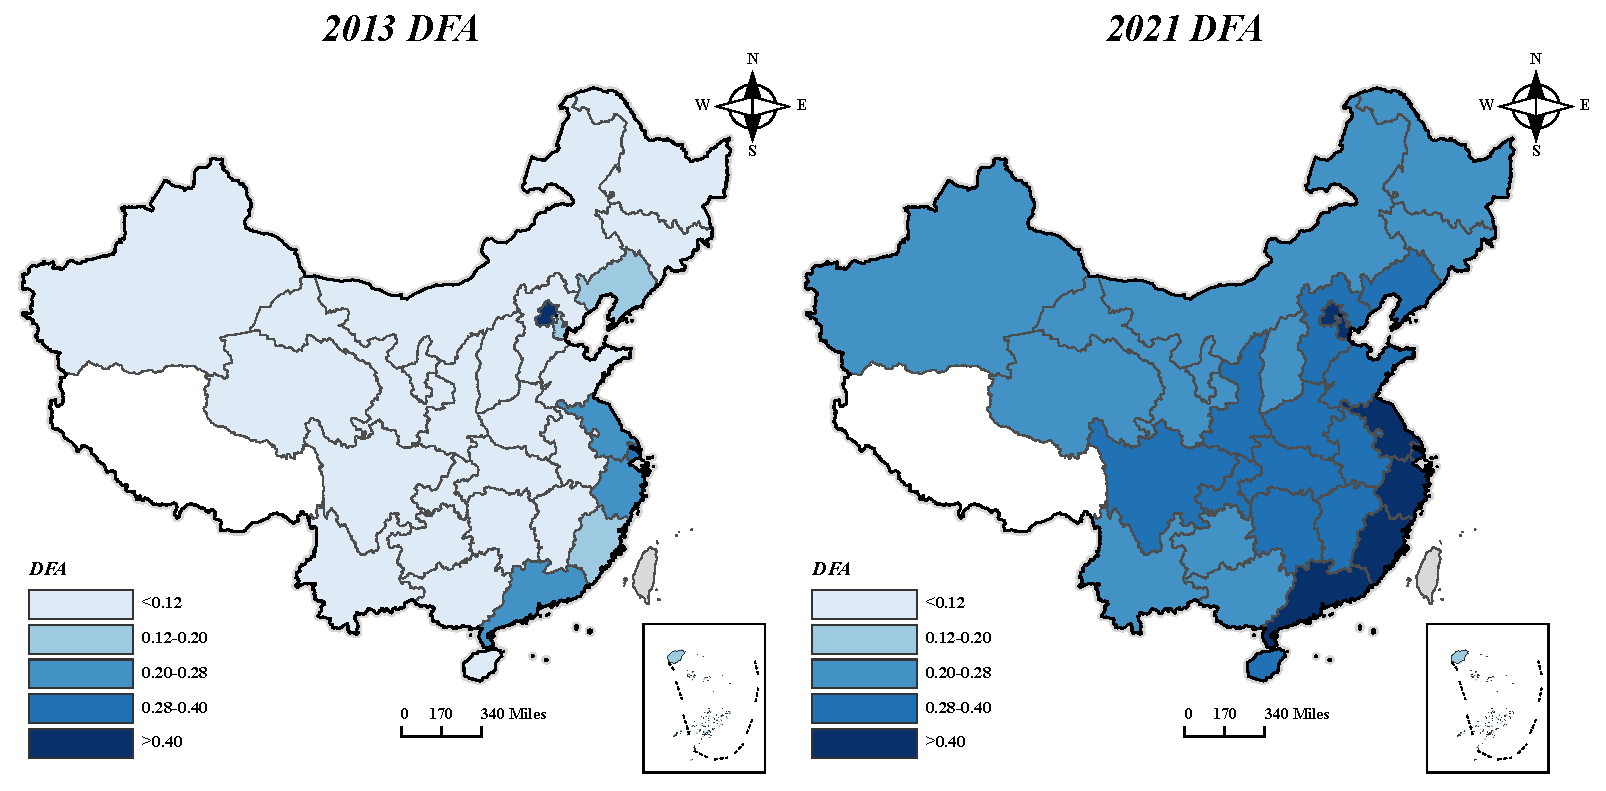
\includegraphics[width=\textwidth]{figures/fig2a_dfa_map_2p.pdf}\\[2pt]
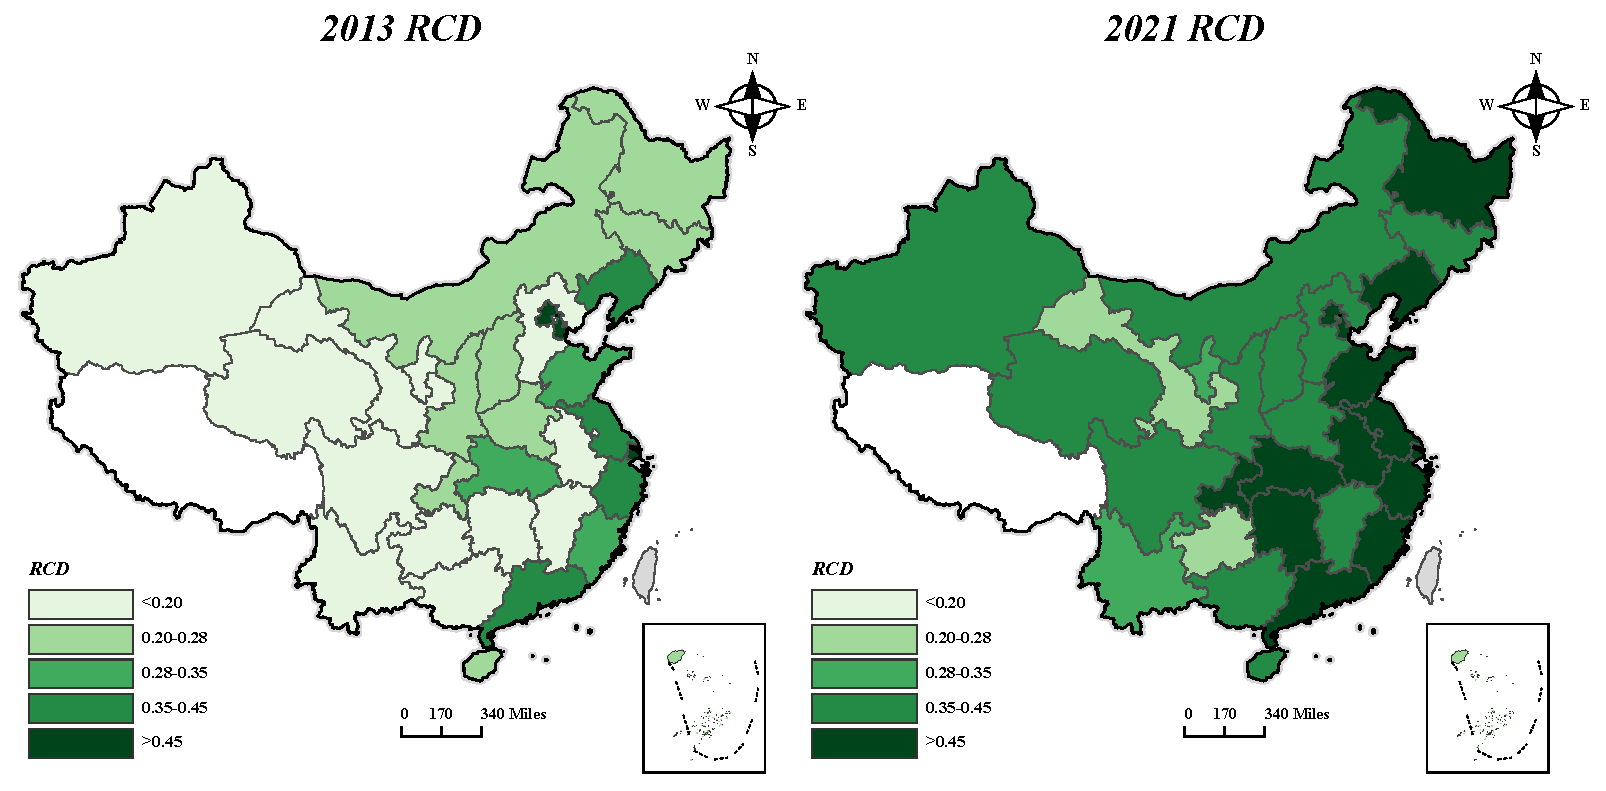
\includegraphics[width=\textwidth]{figures/fig2b_rcd_map_2p.pdf}
\caption{Spatial distribution of DFA and RCD, 2013 and 2021. (a) DFA; (b) RCD. Tibet is shown in white and Taiwan in light gray because they are not included in the estimation sample. The five classes use fixed cutoffs for comparability across years.}\label{fig:maps}
\end{figure}

Figure~\ref{fig:trends} shows the regional averages over time. The eastern region maintains a clear lead in both indices. The western region starts from the lowest level but grows faster in DFA, especially after 2015. The northeastern region has a relatively high initial RCD but a slow digital transition, and its RCD growth is modest. These regional trajectories are consistent with the heterogeneity analysis in Section~\ref{sec:heterogeneity}.

\begin{figure}[H]
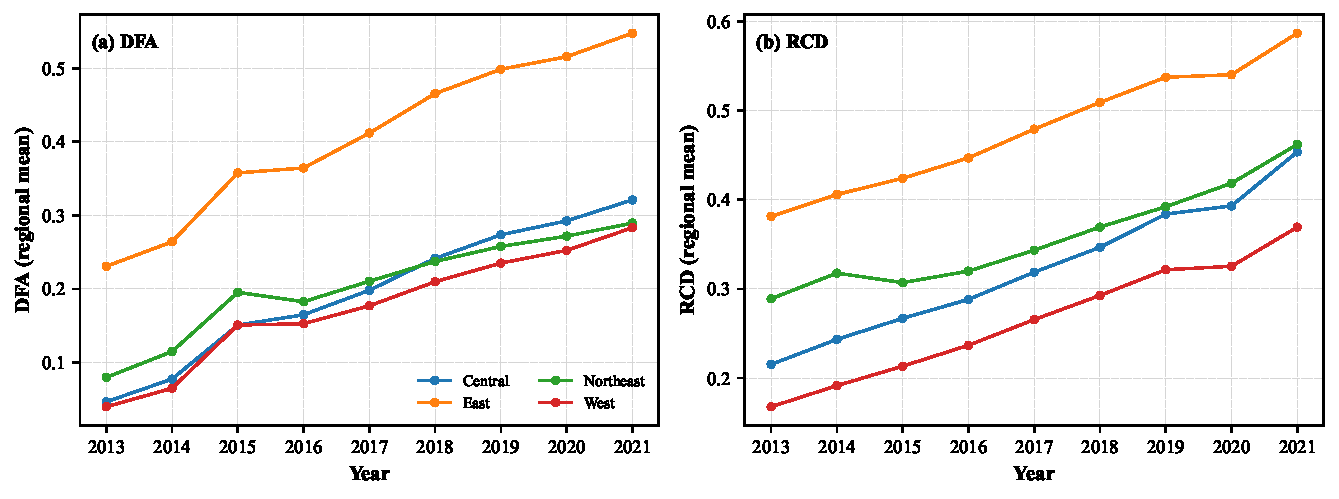
\includegraphics[width=\textwidth]{figures/fig6_trends.pdf}
\caption{Regional averages of DFA and RCD, 2013--2021. (a) DFA; (b) RCD. Regions are defined as East, Central, West, and Northeast.}\label{fig:trends}
\end{figure}

\subsection{Baseline Estimates}\label{sec:baseline}

Table~\ref{tab:baseline} reports the baseline estimates. Column (1) includes DFA without controls and with province and year fixed effects. The coefficient is 0.277 and is significant at the 5\% level. Column (2) adds the four controls. The coefficient falls to 0.241 but remains significant at the 5\% level. Column (3) adds region-specific linear trends to absorb differential regional trends. The coefficient is 0.204 and is significant at the 10\% level. Column (4) uses the five-dimension RCD index as the outcome; the coefficient is 0.013 and is not statistically significant.

The baseline estimate implies that a one-unit increase in the DFA index is associated with an increase of 0.241 points in the RCD index, or about 1.6 standard deviations of RCD. Since the DFA index ranges from 0 to 1, this is a large effect at the upper end of the distribution. A more modest increase of one standard deviation in DFA (0.179) is associated with an increase of about 0.043 points in RCD, or 0.29 standard deviations. The estimate is therefore economically meaningful as well as statistically significant.

The controls are generally insignificant. Government intervention, FDI, population density, and private economy vitality do not have robust associations with RCD once province and year fixed effects are included. This is not surprising: the controls are intended to absorb local conditions, not to explain RCD. Their inclusion does not change the DFA coefficient much, which suggests that the baseline result is not driven by these observable confounders.

The contrast between columns (2) and (4) is informative. DFA is positively associated with the three core coordination dimensions but not with the extended five-dimension index. The extended index adds infrastructure and ecological coordination, which are slower-moving and may respond to digitalization with a longer lag. The result suggests that the short-run effect of DFA operates mainly through economic, social, and urban-rural coordination, not through infrastructure or ecological outcomes. We return to this point in the robustness discussion.

\begin{table}[H]
\caption{Baseline estimates of the effect of DFA on RCD.}\label{tab:baseline}
\begin{threeparttable}
\small
\begin{tabular}{lrrrr}
\toprule
 & (1) & (2) & (3) & (4) \\
\midrule
DFA & 0.277** & 0.241** & 0.204* & 0.013 \\
 & (0.112) & (0.118) & (0.118) & (0.133) \\[2pt]
Government intervention &  & -0.0012 & -0.0007 & -0.0001 \\
 &  & (0.001) & (0.001) & (0.001) \\[2pt]
Log FDI &  & 0.0215 & 0.0169 & 0.0183 \\
 &  & (0.016) & (0.017) & (0.013) \\[2pt]
Log population density &  & 0.0794 & 0.1483 & 0.1003 \\
 &  & (0.138) & (0.203) & (0.129) \\[2pt]
Private economy &  & -0.00002 & 0.00011 & -0.00016 \\
 &  & (0.000) & (0.000) & (0.000) \\[2pt]
Controls & No & Yes & Yes & Yes \\
Province FE & Yes & Yes & Yes & Yes \\
Year FE & Yes & Yes & Yes & Yes \\
Region trends & No & No & Yes & No \\
Observations & 270 & 270 & 270 & 270 \\
\bottomrule
\end{tabular}
\begin{tablenotes}
\small
\item Notes: The dependent variable is RCD in columns (1)--(3) and RCD5 in column (4). DFA is the digital factor allocation index. Controls include government intervention, log FDI per capita, log population density, and private economy vitality. Province and year fixed effects are included in all columns. Region trends are region-specific linear trends. Standard errors clustered by province are in parentheses. $^{***}p<0.01$, $^{**}p<0.05$, $^{*}p<0.10$.
\end{tablenotes}
\end{threeparttable}
\end{table}

\subsection{Threshold Estimates}\label{sec:threshold}

Table~\ref{tab:threshold} reports the threshold tests and regime coefficients. Panel A shows the estimated threshold, the 95\% likelihood-ratio confidence interval, the $F$ statistic for the null of linearity, and the bootstrap $p$-value. Panel B shows the low- and high-regime coefficients of DFA.

The economic-development threshold is the main result. The estimated threshold is 10.589 in log GDP per capita, which corresponds to about CNY 39,700 per person. The bootstrap $p$-value is 0.003, so the null of linearity is rejected at the 1\% level. The low-regime coefficient is 0.506 and the high-regime coefficient is 0.677; both are significant at the 1\% level. The estimated marginal association is therefore about 34\% larger after economic development crosses the threshold. Because the threshold model absorbs only province fixed effects, its coefficients are not directly comparable to the two-way fixed-effects estimates in Table~\ref{tab:baseline}; the relevant comparison is between the low and high regimes within the threshold model. This pattern is consistent with H2 and with the absorptive-capacity interpretation: digital factor allocation is more effective when local income, markets, and complementary capabilities are sufficiently developed.

Figure~\ref{fig:lr} plots the likelihood-ratio statistic for the economic-development threshold. The minimum is sharp, and the 95\% confidence interval is narrow, ranging from 10.583 to 10.639. Figure~\ref{fig:scatter} shows the raw association between DFA and RCD, split by the threshold. The high-development regime has a steeper slope, although the raw scatter also reflects the strong cross-sectional correlation between the two indices. The threshold estimate is therefore best read together with the fixed-effects estimates in Table~\ref{tab:baseline}, which absorb time-invariant province characteristics.

\begin{table}[H]
\caption{Threshold tests and regime-specific coefficients.}\label{tab:threshold}
\begin{threeparttable}
\small
\textit{Panel A: Threshold tests}\\[2pt]
\begin{tabular}{lcccc}
\toprule
Threshold variable & $\hat{\gamma}$ & 95\% CI & $F$ & Bootstrap $p$ \\
\midrule
DFA & 0.178 & [0.153, 0.349] & 15.50 & 0.137 \\
ln(per capita GDP) & 10.589 & [10.583, 10.639] & 29.07 & 0.003 \\
Financial development & 10.045 & -- & 61.48 & 0.010 \\
Technological investment & 0.856 & [0.856, 0.998] & 22.70 & 0.120 \\
Private economy vitality & 368.402 & [85.480, 368.402] & 23.81 & 0.107 \\
\bottomrule
\end{tabular}\par\vspace{8pt}
\textit{Panel B: Regime-specific coefficients of DFA}\\[2pt]
\begin{tabular}{lccc}
\toprule
Threshold variable & Low regime & High regime & Observations (low/high) \\
\midrule
DFA & 0.549*** & 0.661*** & 90/180 \\
 & (0.060) & (0.066) & \\[2pt]
ln(per capita GDP) & 0.506*** & 0.677*** & 66/204 \\
 & (0.057) & (0.067) & \\[2pt]
Financial development & 0.578*** & 0.267*** & 240/30 \\
 & (0.065) & (0.082) & \\[2pt]
Technological investment & 0.812*** & 0.627*** & 33/237 \\
 & (0.088) & (0.051) & \\[2pt]
Private economy vitality & 0.652*** & 0.573*** & 244/26 \\
 & (0.066) & (0.070) & \\[2pt]
\bottomrule
\end{tabular}
\begin{tablenotes}
\small
\item Notes: Each row corresponds to a separate threshold model with province fixed effects and the full control set. The threshold is estimated by grid search over the inner 80\% of the threshold variable's distribution. The $F$ statistic tests the null of a single linear regime. The bootstrap $p$-value is based on 300 cluster wild bootstrap replications. Standard errors clustered by province are in parentheses. For financial development, the likelihood-ratio interval collapses at the grid resolution; it is therefore not reported. $^{***}p<0.01$, $^{**}p<0.05$, $^{*}p<0.10$.
\end{tablenotes}
\end{threeparttable}
\end{table}

\begin{figure}[H]
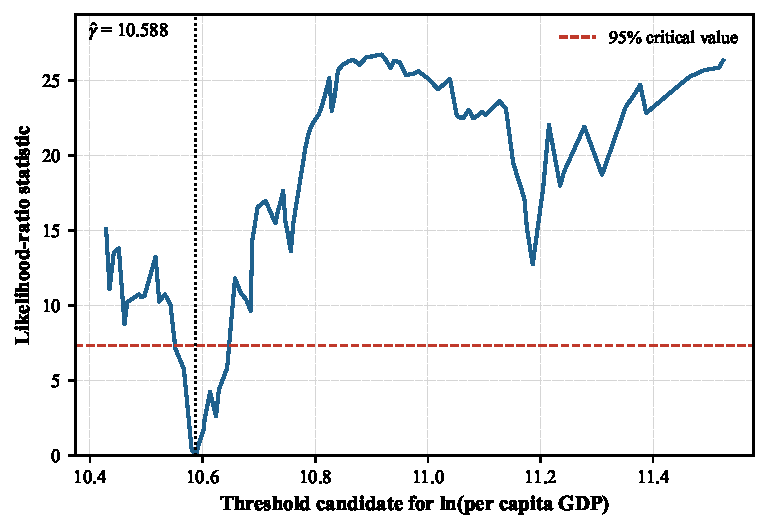
\includegraphics[width=0.68\textwidth]{figures/fig4_lr_curve.pdf}
\caption{Likelihood-ratio statistic for the economic-development threshold. The dashed line is the 95\% critical value (7.35). The dotted vertical line marks the estimated threshold.}\label{fig:lr}
\end{figure}

\begin{figure}[H]
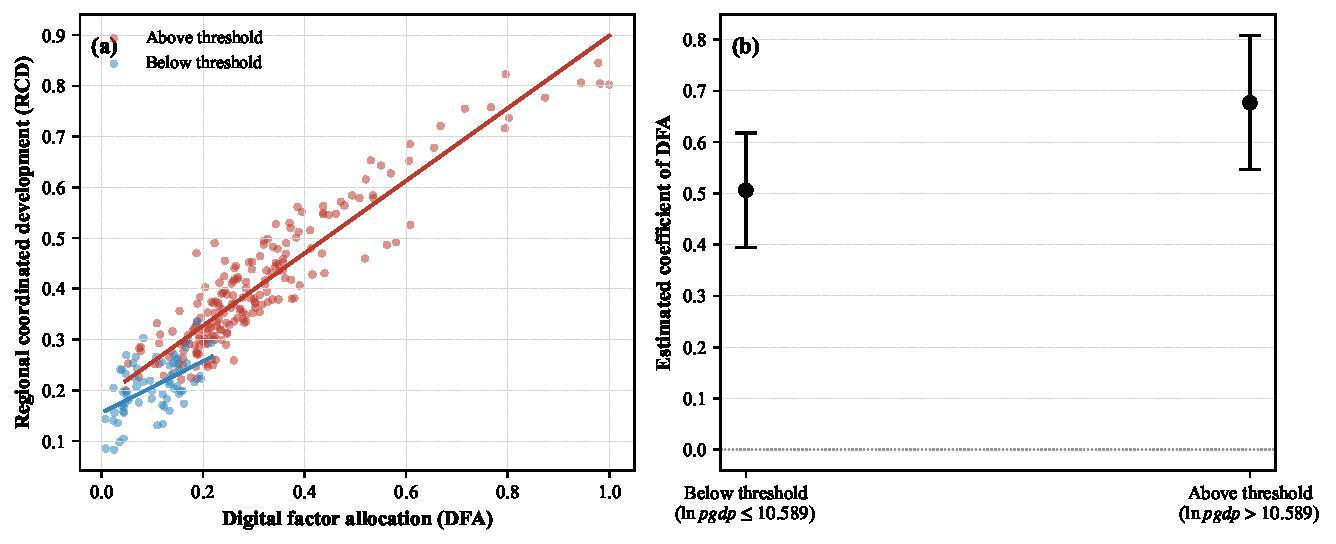
\includegraphics[width=\textwidth]{figures/fig3_scatter_regimes.pdf}
\caption{DFA, RCD, and the economic-development threshold. (a) Raw association between DFA and RCD, split by the estimated threshold; the lines are linear fits within each regime. (b) Regime-specific coefficients of DFA with 95\% confidence intervals from the threshold model.}\label{fig:scatter}
\end{figure}

The financial-development threshold is also statistically significant, but its interpretation requires caution. The estimated threshold is 10.045. The low-regime coefficient is 0.578 and the high-regime coefficient is 0.267; the bootstrap $p$-value is 0.010. The high regime contains 30 observations: 27 from Beijing, Shanghai, and Tianjin, plus three observations from Qinghai. The decline in the marginal effect is therefore driven by a small group of financially deep municipalities. It is consistent with diminishing returns to digital finance, but it should not be read as a general statement about all high-finance provinces.

The other threshold variables do not produce statistically significant breaks. The DFA self-threshold has a bootstrap $p$-value of 0.137, the technology threshold 0.120, and the private-economy threshold 0.107. The point estimates suggest some variation across regimes, but the null of linearity cannot be rejected. The nonlinearity in the data is therefore primarily associated with economic development, not with the level of digitalization itself.

One caveat applies to all threshold estimates. The threshold model follows Hansen (1999) and includes province fixed effects but not year fixed effects. Because the threshold variable is a slow-moving development indicator, year fixed effects would absorb much of the cross-province variation in development stages that identifies the threshold. When region-specific linear trends are added, the economic-development threshold remains positive but becomes statistically weaker (bootstrap $p=0.47$). The threshold should therefore be interpreted as a long-run structural pattern rather than a short-run causal effect. We discuss this limitation further in Section~\ref{sec:limitations}.

\subsection{Regional Heterogeneity}\label{sec:heterogeneity}

Table~\ref{tab:heterogeneity} reports the regional estimates. Under two-way fixed effects, the western region has a positive and highly significant coefficient of 0.555. The eastern and central coefficients are positive but insignificant (0.227 and 0.192), and the northeastern coefficient is negative and insignificant ($-0.223$). Under province fixed effects, all four regions have positive and significant coefficients, with the largest coefficients in the west (0.535) and central region (0.485), followed by the east (0.296) and the northeast (0.096).

The western result is the most robust. It holds under both specifications and is significant at the 1\% level. This is consistent with H4 and with the catch-up interpretation: the marginal return to digital factor allocation is higher in regions that start with lower levels of digital infrastructure and financial access. The eastern and central results are sensitive to the inclusion of year fixed effects, which suggests that their average association is partly driven by common national trends. The northeastern result is weak and sometimes negative, which may reflect the region's industrial legacy and slow digital transition.

The regional pattern should not be overinterpreted. The subsample estimates are less precise than the full-sample estimates, and the differences across regions are not formally tested. The results are best read as descriptive evidence that the DFA--RCD relationship is not uniform across China's regions, with the west showing the most consistent positive association.

\begin{table}[H]
\caption{Regional heterogeneity in the effect of DFA on RCD.}\label{tab:heterogeneity}
\begin{threeparttable}
\small
\begin{tabular}{lcc}
\toprule
Region & Two-way FE & Province FE \\
\midrule
East & 0.227 & 0.296*** \\
 & (0.234) & (0.104) \\[2pt]
Central & 0.192 & 0.485*** \\
 & (0.340) & (0.072) \\[2pt]
West & 0.555*** & 0.535*** \\
 & (0.125) & (0.077) \\[2pt]
Northeast & -0.223 & 0.096*** \\
 & (0.285) & (0.023) \\[2pt]
Controls & Yes & Yes \\
Observations & 90/54/99/27 & 90/54/99/27 \\
\bottomrule
\end{tabular}
\begin{tablenotes}
\small
\item Notes: Each cell reports the coefficient of DFA from a separate regression for the indicated region. Controls are included in all columns. Two-way FE includes province and year fixed effects; province FE includes province fixed effects only. Standard errors clustered by province are in parentheses. $^{***}p<0.01$, $^{**}p<0.05$, $^{*}p<0.10$.
\end{tablenotes}
\end{threeparttable}
\end{table}

\subsection{Robustness}\label{sec:robustness}

Table~\ref{tab:robustness} reports the robustness checks. The baseline coefficient is 0.241. It remains positive and significant when the RCD index is replaced by a globally entropy-weighted index (0.349), when the DFA index is replaced by an equal-weight indicator index (0.298), when municipalities are excluded (0.288), when the sample ends in 2019 (0.283), and when the outcome and regressor are winsorized at the 1st and 99th percentiles (0.302). The coefficient is larger under province fixed effects (0.689) and smaller and insignificant when the five-dimension RCD index, the coupling coordination degree, the entropy-weighted DFA index, or lagged DFA are used.

The pattern is informative. The positive effect is robust to alternative weighting of the RCD indicators and to the exclusion of the largest municipalities. It is also robust to dropping 2020, which suggests that the COVID-19 shock is not driving the result. The effect is weaker for the five-dimension RCD index and for the coupling coordination degree. This is consistent with the baseline contrast in Table~\ref{tab:baseline}: the five-dimension index adds infrastructure and ecological dimensions that are less responsive to DFA in the short run, and the coupling coordination degree emphasizes balance among dimensions rather than levels.

The insignificant coefficient for lagged DFA suggests that the effect is contemporaneous rather than delayed. This may reflect the fast diffusion of digital services: once infrastructure and platforms are available, their coordination effects appear within the same year. It may also reflect measurement: the DFA index captures the current state of digital factor allocation, and its effect on RCD is likely to be strongest when the digital environment is contemporaneous with economic and social outcomes.

The entropy-weighted DFA index produces a positive but insignificant coefficient. This index places more weight on IPv4 addresses and domain names, which are concentrated in a few leading provinces. The equal-weight index and the baseline index, which give more balanced weight to infrastructure, industry, finance, and human capital, produce stronger results. This suggests that the effect is not driven by a single digital indicator but by the combined allocation of digital factors.

\begin{table}[H]
\caption{Robustness checks.}\label{tab:robustness}
\begin{threeparttable}
\small
\begin{tabular}{lccc}
\toprule
Specification & Coefficient & SE & N \\
\midrule
Baseline & 0.241** & (0.118) & 270 \\
Five-dimension RCD & 0.013 & (0.133) & 270 \\
CCD of core dimensions & 0.118 & (0.288) & 270 \\
Entropy-weighted RCD & 0.349** & (0.154) & 270 \\
Equal-weight DFA & 0.298** & (0.143) & 270 \\
Entropy-weighted DFA & 0.186 & (0.176) & 270 \\
Excluding municipalities & 0.288** & (0.128) & 234 \\
2013-2019 & 0.283** & (0.123) & 210 \\
Additional controls & 0.213 & (0.138) & 270 \\
Province FE only & 0.689*** & (0.069) & 270 \\
Lagged DFA & 0.139 & (0.146) & 240 \\
Winsorized 1/99 & 0.302** & (0.122) & 270 \\
\bottomrule
\end{tabular}
\begin{tablenotes}
\small
\item Notes: Each row reports the coefficient of DFA (or lagged DFA) from a separate regression. The baseline includes the full control set and two-way fixed effects. The five-dimension RCD index adds infrastructure and ecological coordination. The coupling coordination degree is computed from the three core dimensions. The equal-weight DFA index uses equal weights for all 15 indicators. The entropy-weighted DFA index uses global entropy weights. The additional-controls specification adds technological investment, industrial structure upgrading, and financial development. Standard errors clustered by province are in parentheses. $^{***}p<0.01$, $^{**}p<0.05$, $^{*}p<0.10$.
\end{tablenotes}
\end{threeparttable}
\end{table}

\begin{figure}[H]
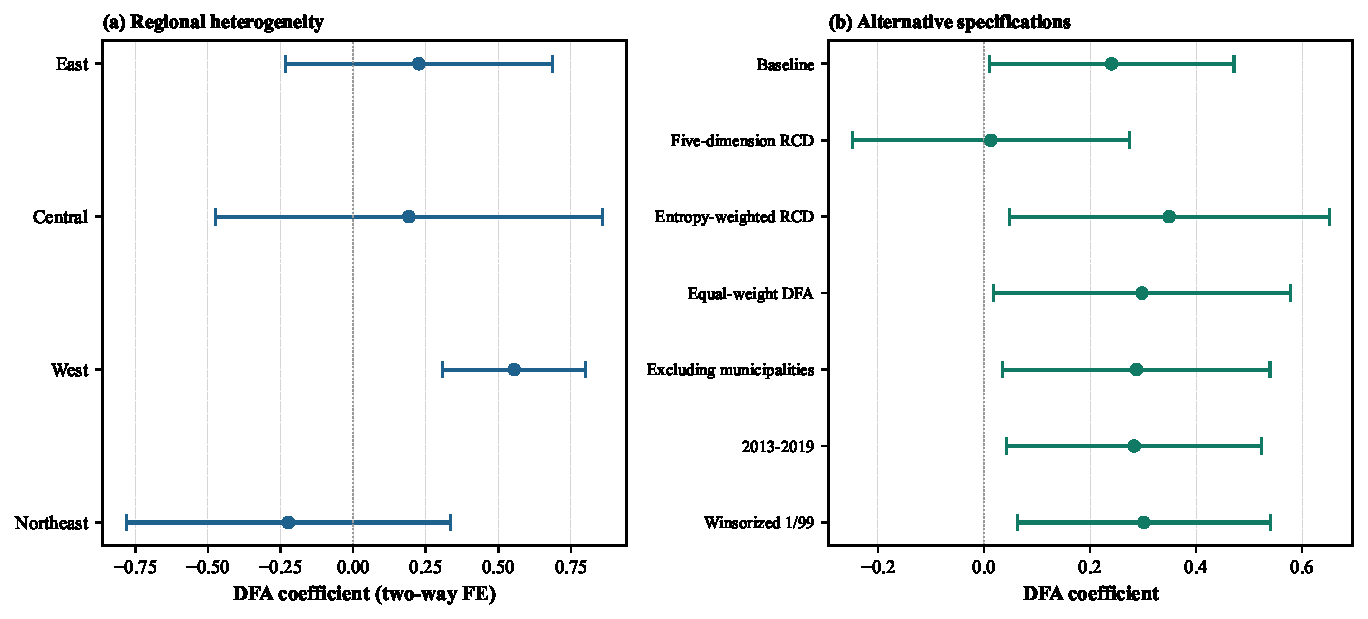
\includegraphics[width=\textwidth]{figures/fig5_coefficients.pdf}
\caption{Regional and specification heterogeneity. (a) Regional DFA coefficients under two-way fixed effects. (b) DFA coefficients under alternative specifications. Bars are 95\% confidence intervals.}\label{fig:coef}
\end{figure}

\subsection{Mechanisms}\label{sec:mechanisms}

Table~\ref{tab:mechanisms} reports the channel regressions. DFA is positively associated with technological investment (6.290, p < 0.05) and financial development (8.885, p < 0.01) under two-way fixed effects, and with industrial structure upgrading under province fixed effects (144.903, p < 0.01). These results are consistent with the view that digital factor allocation supports RCD through innovation, financial deepening, and structural change.

The income-gap result is more nuanced. Under two-way fixed effects, DFA is positively associated with the urban-rural income ratio (0.715, p < 0.05), which implies that a one-unit increase in DFA widens the urban-rural income gap in the short run. Under province fixed effects, the association is negative ($-1.279$, p < 0.01), which implies that over the longer run digital factor allocation is associated with a narrower gap. The contrast suggests that the distributional effect of digitalization is horizon-dependent: in the short run, digital opportunities may be captured disproportionately by urban and skilled groups, while in the longer run, the diffusion of digital services to rural areas may narrow the gap.

The mediator coefficients in the RCD equation are not statistically significant. This means that the channel evidence should be read as suggestive rather than as a formal mediation analysis. The reduced-form effect of DFA on RCD remains positive when the mediators are included, which suggests that the channels complement rather than fully explain the relationship. A more complete mediation analysis would require exogenous variation in each channel, which is beyond the scope of this study.

\begin{table}[H]
\caption{Channel regressions.}\label{tab:mechanisms}
\begin{threeparttable}
\small
\resizebox{\textwidth}{!}{\begin{tabular}{lccc}
\toprule
Mediator & DFA $\to$ M (two-way FE) & DFA $\to$ M (province FE) & M in RCD equation \\
\midrule
Technological investment & 6.290** & 1.255 & 0.006 \\
 & (2.985) & (1.275) & \\[2pt]
Financial development & 8.885*** & 4.941*** & -0.001 \\
 & (3.164) & (1.773) & \\[2pt]
Industrial upgrading & 127.226 & 144.903*** & -0.000 \\
 & (80.849) & (29.771) & \\[2pt]
Urban-rural income ratio & 0.715** & -1.279*** & -- \\
 & (0.302) & (0.180) & \\[2pt]
Controls & Yes & Yes & Yes \\
Observations & 270 & 270 & 270 \\
\bottomrule
\end{tabular}}
\begin{tablenotes}
\small
\item Notes: The first two columns report the effect of DFA on the mediator under two-way and province fixed effects, respectively. The third column reports the coefficient of the mediator in the RCD equation. Controls are included in all columns. Standard errors clustered by province are in parentheses. $^{***}p<0.01$, $^{**}p<0.05$, $^{*}p<0.10$.
\end{tablenotes}
\end{threeparttable}
\end{table}

\section{Discussion}\label{sec:discussion}

\subsection{Main Findings}

This study asked whether digital factor allocation promotes regional coordinated development and whether the relationship is nonlinear. The answer is yes on both counts, with qualifications. On average DFA is positively associated with RCD, and the estimate of 0.241 survives alternative weighting of the outcome, the exclusion of municipalities and of 2020, and winsorization. The association is stronger in provinces that have crossed a critical level of economic development and is concentrated in the west. A financial-development threshold indicates declining returns at very high levels of financial depth, although that result rests on a small group of municipalities.

Three points follow for the literature. First, the digital dividend is conditional: digital inputs are more productive when they can be combined with skills, markets, and institutions. Second, the digital-divide and digital-dividend views are both right at different stages of development: access without absorptive capacity does not convert into coordination gains, and once the capacity is in place the same inputs do more. Third, a composite index conceals divergent behaviour across its components. Digital finance carries most of the association, while industrial digitalization and digital human capital change sign across the threshold.

The spatial analysis narrows the claim. The positive association holds in every specification and in both regimes, and the threshold location is stable when the outcome is allowed to depend on neighbouring outcomes. The size of the gap between regimes is not stable. The threshold therefore describes a development gradient in the cross-section, not a sharp structural boundary.

\subsection{Absorptive Capacity and the Digital Divide}

The economic-development threshold is consistent with absorptive capacity. Digital technologies are general-purpose technologies whose effects depend on organizational change, human capital, and complementary infrastructure \citep{brynjolfsson2014,omahony2005}. In low-income provinces digital infrastructure may be used mainly for communication and consumption, while productive and coordination effects require inputs that are in short supply. In higher-income provinces digital inputs can be combined with skilled labour, financial services, and market institutions.

This is also consistent with the multi-level digital divide. Access is the first level, skills the second, and the ability to convert access into material benefits the third \citep{vandijk2005,norris2001,warschauer2003}. Our results suggest that the third-level divide binds in low-income provinces, so providing access alone is not enough.

The regional and threshold results are not in conflict. The regional estimate compares average outcomes across regions over the sample period, while the threshold estimate compares provinces at different development stages within a period. The west can have a larger average association because it starts from a lower base even if the marginal association at a given development level is smaller.

\subsection{Financial Development and Diminishing Returns}

The financial-development threshold suggests that the marginal association of DFA declines at very high levels of financial depth, consistent with diminishing returns to digital finance at the extensive margin. Where financial systems are shallow, digital finance expands access to basic services; where they are deep, it adds less to access and may instead intensify competition or encourage speculative activity \citep{beck2007}. The result rests on 30 high-regime observations, mostly Beijing, Shanghai, and Tianjin, and should be read as a caution against assuming that more digital finance always produces more coordination.

The decomposition of the index points at the same factor from another direction. Entered jointly, digital finance is the only dimension with an independent association with RCD, and its regime pattern mirrors the composite: positive in both regimes and slightly larger above the threshold. Financial depth therefore matters twice, as a moderator of the association and as the carrier of most of it. The two roles are conceptually distinct but point to the same policy margin: the quality and direction of digital finance rather than its volume.

\subsection{Regional Heterogeneity}

The association is strongest in the west and weaker or insignificant elsewhere under two-way fixed effects, which supports the inclusive-digitalization view: where digital infrastructure and financial access are scarce, additional digital factors have larger marginal effects. The northeast is weaker and sometimes negative. It has relatively high initial urbanization and public services but a slow digital transition and a declining working-age population, so digital factor allocation may not offset these structural constraints without a broader revitalization strategy.

\subsection{Policy Implications}

Digital factor allocation should be sequenced with economic development. In low-income provinces the priority is basic connectivity, digital literacy, and complementary public services; advanced digital industry and digital finance are unlikely to raise coordination until those foundations are in place. In higher-income provinces the priority shifts to deeper integration of digital technologies into production, public services, and urban-rural linkages.

Policies should be tailored to regional absorptive capacity. The west has the strongest average association and should be a priority for digital infrastructure and digital finance investment, paired with human capital development and market reform. Because the short-run association with the urban-rural income ratio is positive, gains may be captured disproportionately by urban and skilled groups; rural e-commerce, digital agriculture, digital public services, and targeted skills training can broaden them. Advanced regions should attend to the quality and direction of digital investment rather than its quantity, given the declining association at high financial depth.

\subsection{Limitations}\label{sec:limitations}

Four limitations deserve emphasis. First, the analysis covers 30 provinces and does not capture within-province heterogeneity; city-level data would provide a more granular picture. Second, the indices depend on indicator selection and weighting. We use alternative weighting schemes and alternative outcome definitions, but the indices remain simplifications.

Third, the estimates are conditional associations. DFA may be endogenous to RCD, and the lagged specification is not significant, which suggests a contemporaneous relationship that could reflect reverse causality. Oster bounds and the randomisation placebo indicate that unobservables would have to be more important than the observed controls to eliminate the association, but they do not identify a causal effect. External instruments such as historical telephone penetration, terrain ruggedness, or distance to the backbone network are not available for this sample, and we do not construct a pseudo-instrument from the index components. Future work should exploit such variation.

Fourth, the threshold is sensitive to specification. Region-specific trends, year fixed effects, and spatial specifications either reduce its precision or move its location, and the size of the break is not stable across spatial models. The threshold should be read as a long-run pattern, not a short-run causal effect. The sub-dimension slopes are also imprecise because the low-income regime contains 66 observations, and the income series carry measurement error from the household survey and from the urban-rural classification. Finally, the sample includes the COVID-19 period; the results are robust to dropping 2020, but 2021 may still be affected.

\section{Conclusions}\label{sec:conclusion}

This study constructed a four-dimension DFA index covering digital infrastructure, digital industry, digital finance, and digital human capital, and a three-dimension RCD index covering economic, social, and urban-rural coordination, for 30 Chinese provinces from 2013 to 2021. Using a Hansen panel threshold model, it tested whether the effect of DFA on RCD depends on economic development and financial development, and it examined which dimension carries the association and whether the estimates survive spatial dependence.

DFA is positively associated with RCD. The baseline two-way fixed-effects estimate is 0.241 and the association holds across alternative weighting, sample restrictions, and winsorization. It is economically meaningful: a one-standard-deviation increase in DFA is associated with an increase of about 0.043 points in RCD, or 0.29 standard deviations.

The association rises with economic development. Above the estimated threshold of 10.589 in log GDP per capita (about CNY 39,700), the marginal association is 0.677 against 0.506 below, consistent with absorptive capacity. A financial-development threshold indicates declining returns at very high levels of financial depth, driven by a small group of financially deep municipalities. Both indices are spatially clustered; allowing for spatial dependence leaves the threshold location unchanged, so we read it as a development gradient rather than a sharp break.

Two findings extend the usual account. Within the composite, digital finance is the only dimension with an independent association, and it also shows the most stable positive slope across regimes. Industrial digitalization and digital human capital, by contrast, switch from negative below the threshold to positive above it, which is what an absorptive-capacity argument predicts. The regional analysis shows the association concentrated in the west, where digital infrastructure and financial access start low.

These findings imply a differentiated policy. Digital factor allocation should be sequenced with economic development: basic connectivity and digital literacy first in low-income provinces, deeper integration of digital technologies into production and public services in higher-income ones. The west should be a priority for digital infrastructure and digital finance investment, paired with human capital development and market reform. Because the short-run association with the urban-rural income ratio is positive, complementary rural digital services and targeted skills training are needed to share the gains. Advanced regions should focus on the quality and direction of digital investment rather than its quantity.

Several limitations remain. The analysis uses provincial data and does not capture within-province heterogeneity; the indices depend on indicator and weighting choices; and the estimates are conditional associations rather than identified causal effects. The threshold is sensitive to the treatment of trends, year effects, and spatial dependence. Future work can address these points with city-level data, external instruments, dynamic spatial threshold models, and a DFA index extended to data governance, digital security, and the quality of digital public services.

Digitalization is not a universal remedy for regional disparities. Its payoff depends on the stage of economic development, the depth of the financial system, and regional absorptive capacity, and a differentiated approach that combines digital investment with complementary economic and social reforms is more likely to deliver inclusive coordination gains.


\vspace{6pt}
\noindent\textbf{Author Contributions:} Conceptualization, J.W. (Junfeng Wang) and Y.W.; methodology, J.W. (Junfeng Wang); formal analysis, J.W. (Junfeng Wang); data curation, J.W. (Jiayi Wang); writing---original draft, J.W. (Junfeng Wang); writing---review and editing, J.W. (Jiayi Wang) and Y.W. All authors have read and agreed to the published version of the manuscript.

\vspace{6pt}
\noindent\textbf{Funding:} This research received no external funding.

\vspace{6pt}
\noindent\textbf{Institutional Review Board Statement:} Not applicable.

\vspace{6pt}
\noindent\textbf{Informed Consent Statement:} Not applicable.

\vspace{6pt}
\noindent\textbf{Data Availability Statement:} The provincial panel data are compiled from publicly available official yearbooks and the Peking University Digital Financial Inclusion Index. The analysis panel and replication code are available from the corresponding author upon reasonable request.

\vspace{6pt}
\noindent\textbf{Conflicts of Interest:} The authors declare no conflict of interest.

\appendix
\setcounter{section}{0}
\setcounter{table}{0}
\renewcommand{\thetable}{A\arabic{table}}
\section{Index Weights}\label{app:weights}

Table~\ref{tab:weights} reports the within-dimension entropy weights for DFA and the global entropy weights for RCD. The DFA index assigns equal weights to the four dimensions. The RCD baseline assigns equal weights to the three dimensions; the weights below refer to the global entropy-weighted alternative used in the robustness checks.

\begin{table}[H]
\caption{Entropy weights for DFA and RCD indicators.}\label{tab:weights}
\begin{threeparttable}
\small
\begin{tabular}{llc}
\toprule
Dimension & Indicator & Weight \\
\midrule
\multicolumn{3}{l}{\textit{Panel A: DFA (equal weights across four dimensions)}} \\
Digital infrastructure & Internet access ports per capita & 0.057 \\
Digital infrastructure & Optical cable density & 0.211 \\
Digital infrastructure & Mobile phone penetration & 0.056 \\
Digital infrastructure & IPv4 addresses per capita & 0.414 \\
Digital infrastructure & Domain names per capita & 0.262 \\
Digital industry & Software revenue/GDP & 0.336 \\
Digital industry & E-commerce sales/GDP & 0.214 \\
Digital industry & Share of firms with e-commerce & 0.085 \\
Digital industry & Websites per 100 firms & 0.042 \\
Digital industry & Information firms per capita & 0.323 \\
Digital finance & DFI coverage breadth & 0.303 \\
Digital finance & DFI usage depth & 0.376 \\
Digital finance & DFI digitization & 0.322 \\
Digital human capital & ICT employment share & 0.762 \\
Digital human capital & Internet penetration & 0.238 \\
\midrule
\multicolumn{3}{l}{\textit{Panel B: RCD (global entropy weights)}} \\
Economic & GDP per capita & 0.157 \\
Economic & Retail sales per capita & 0.156 \\
Economic & Fiscal self-sufficiency & 0.084 \\
Social & Disposable income per capita & 0.150 \\
Social & Hospital beds per 10,000 & 0.080 \\
Social & Higher-education students per 100,000 & 0.073 \\
Social & Social security spending share & 0.102 \\
Urban-rural & Urbanization rate & 0.081 \\
Urban-rural & Urban-rural income ratio (negative) & 0.049 \\
Urban-rural & Urban unemployment rate (negative) & 0.066 \\
\bottomrule
\end{tabular}
\begin{tablenotes}
\small
\item Notes: Panel A reports within-dimension entropy weights for DFA; each of the four dimensions receives a weight of 0.25 in the composite. Panel B reports global entropy weights for the ten RCD indicators, used in the entropy-weighted RCD robustness check.
\end{tablenotes}
\end{threeparttable}
\end{table}

\bibliography{references}

\end{document}
